% !TEX root = main.tex

\section{はじめに}
ムーアの法則の終焉により,CPUのコア単体性能は限界に達しつつある.
一方で,IT技術の発展に伴い管理すべきデータは爆発的に増えつつある.
この状況に対処するため,現在のコンピュータ技術は複数のコアを用いて処理を行うマルチスレッド処理が主流である.
データベース分野においても例外ではなく,近年メニーコアなどを前提としたインメモリデータベースの研究が進んでいる.
データベースの構成要素の1つである索引技術も同様に,メニーコア・大容量メモリに適合させる必要がある.

代表的な索引構造である\Bptree{}~\cite{book:dbsystem}では,ロックを用いた同時実行制御が行われている.
しかし,マルチスレッド処理においてロックによる同時実行制御は多数の待ちスレッドが発生するため,スケーラビリティが悪化する.
そこで,\Bptree{}をロックフリー化させた索引としてBw木~\cite{book:Bwtree}やBz木~\cite{book:Bztree},著者らの研究室で開発しているロックフリーB+木(\Bctree{})が提案されている.

また,インターネットの普及に伴いURLの管理やECサイトにおける文字列検索など,特定のキーに対し効率的に処理する索引構造が求められている.
Mass木~\cite{book:Masstree}は,文字列型や整数型などのバイナリ比較可能なキーに特化した索引構造の1~つである.
\Bptree{}を階層的に作成することにより,キャッシュ効率を改善している.

本研究の\Bcforest{}では,著者らの研究室で開発しているロックフリーB+木(\Bctree{})に対し,Mass木のと同様の拡張および性能改善を行う.
Mass木の観点では\Bptree{}から\Bctree{}になることにより,ロックフリーによる書き込み性能の改善を図る.
また,Posting listの利用により,Mass木における空間利用率の改善を図る.
\Bctree{}の観点では,整数型や文字列型などのバイナリ比較可能なキーに対し,キャッシュ効率の改善を図る.


本稿の構成は以下の通りである.
\Sec{\ref{sec:relatedwork}}では,関連研究としてロックフリー索引やバイナリ比較可能なキーに対し最適化した索引について概説する.
次に,\Sec{\ref{sec:bc_forest_structure}}で\Bcforest{}の構造について説明し,\Sec{\ref{sec:node_operation}}および\Sec{\ref{sec:smo}}で\Bcforest{}の操作について述べる.
最後に,\Sec{\ref{sec:conclusion}}で本稿のまとめと今後の方針を述べる.

\section{関連研究}
\label{sec:relatedwork}
関連の深い索引構造として,同時実行制御においてロックを取得しない\Bctree{},および\Bptree{}にトライ木の構造を組み合わせたMass木について紹介する.

\subsection{\Bctree{}}
\Bctree{}はマッピングテーブル・ノード内バッファという構造上の特徴を持ち,これらの構造およびCAS命令を利用することで大部分の操作をロックフリー化した索引である.
\Bctree{}の概形を\Fig{\ref{fig:bc_tree-structure}}に示す.

\begin{figure}[t]
    \centering
    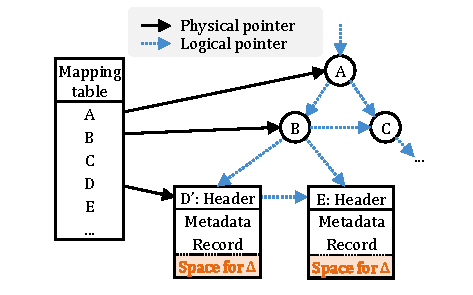
\includegraphics{./figures/Bc-structure.pdf}
    \caption{\Bctree{}の概形}
    \label{fig:bc_tree-structure}
\end{figure}

\subsubsection{データ構造の概観}
\Bptree{}と同様に,\Bctree{}は索引層およびデータ層によって構成される.
索引層のノード(中間ノード)は分割キーと子ノードへのポインタの組を格納し,木の下方への検索を補助する.
構造は\Blinktree{}に則っており,各ノードが同じ階層の右兄弟への参照リンクを持つ.

ノード間の繋がりはマッピングテーブルにより仮想化する.
各ノードは自身の子ノードや兄弟ノードへのポインタを直接持つ代わりにマッピングテーブル上のID(logical page ID, LPID)を持つ.
各ノードへの参照はマッピングテーブルを用いた間接参照を採用し,マッピングテーブル内の物理ポインタを差し替えることでそのノードへの参照を一括で変更する.

各ノードの領域は不変領域と可変領域(ノード内バッファ)に分けられる.
不変領域はノードヘッダおよびソート済みのレコードを格納する.
ヘッダは不変領域の情報を管理し,構造変更時のみその値が変更される.
可変領域はステータスワードの格納と差分レコードを挿入するための書き込みバッファの役割を果たす.
ステータスワードは可変領域の情報を管理し,ノードの現在の状態や残容量などを管理する.

\subsubsection{レコード操作の概観}
ステータスワードをCAS命令で更新することによって,ロックフリーな書き込みを実現している.
書き込み操作は差分レコード領域の予約とレコード挿入および可視化の2ステップで行われる.
\Fig{\ref{fig:bc_tree_insertion}}に\Bctree{}における差分レコードの挿入を示す.

ノードフッタにはミュータブル領域の状態を表すステータスワードを用意し,この中のレコード数と使用済みブロックサイズを加算することで差分レコード用の領域を予約する.
また,\Bctree{}ではノードの生成時にミュータブル領域をゼロ埋めしている.
\Bctree{}では,メタデータがゼロ埋めされている場合を処理途中として表すため,差分レコード用の領域を予約した時点ではレコードが可視化されていないことを認識できる.
確保した領域へ差分レコードを書き込み,対応するレコードメタデータの値を更新することでレコードを可視化し,挿入処理を完了する.
書き込み同士の競合はステータスワードで解決され,差分レコード用領域の予約,つまり差分レコードの書き込み順はCAS命令の成功順によって順序付けられる.

\begin{figure}[t]
    \centering
    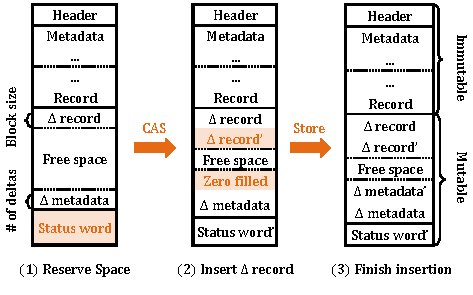
\includegraphics{./figures/Bc-insertion.pdf}
    \caption{\Bctree{}における差分レコードの挿入}
    \label{fig:bc_tree_insertion}
\end{figure}

\subsection{Mass木}
Mass木は\Bptree{}を基本単位とした階層構造やレコードメタデータの削除により,キャッシュ効率を改善した索引構造である.
Mass木の概形を\Fig{\ref{fig:masstree}}に示す.

\begin{figure}[t]
    \centering
    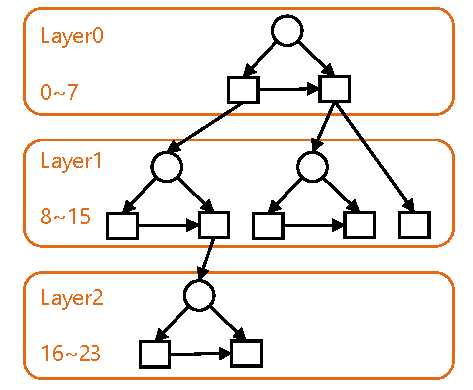
\includegraphics{./figures/masstree.pdf}
    \caption{Mass木の概形}
    \label{fig:masstree}
\end{figure}

Mass木は複数の\Bptree{}とlayer構造から構成される.
Layer~0はキーの先頭0~7~byteで構成される\Bptree{}である.
先頭8~byteで一意性が確保できる場合には,Layer~0で完結する.
先頭8~byteで一意性が確保出来ない場合,Layer~1(キーの8~15~byte目で構成される\Bptree{})を作成し,Layer~0からLayer~1への物理リンクを張る.
同様にして,複数の\Bptree{}やLayerを作成し,トライ木に似た構造を持つのがMass木の特徴である.
Mass木は整数型や文字列型など,分割が可能なキーに限定することで上記に示す階層化(共通部分の集約)を可能にしている.

また,Mass木は固定長キーおよび固定長ペイロードに特化したノードレイアウトを利用している.
\Bctree{}のような可変長キーおよび可変長ペイロードに対応する索引構造では,各レコードに対応するレコードメタデータを利用することでノード内のレコードの配置等を管理している.
一方,Mass木ではキーを8~byte毎に分割するため各階層の\Bptree{}で管理されるキーが8~byte固定長となる.
ペイロードに関しても,可変長のペイロードなどは動的に確保した領域に保持し索引内にはそのポインタのみを格納することで,索引内では全てのペイロードを同じく8~byte固定長で扱う.
つまりレコードの個数などから一意に参照先を決定でき,レコードメタデータの除外とそれによるCPUキャッシュ効率の改善が実現されている.

\section{\Bcforest{}の構造}
\label{sec:bc_forest_structure}

\Bcforest{}は\Bctree{}をバイナリ比較可能なキーに最適化した索引構造である.
Mass木のように8~byte単位でキーを分割,階層分けし,各階層でのレコード管理にはBc木を利用する.
つまり,各Bc木の中間ノードでは固定長の部分キーおよび子ノードへのポインタのみを管理することとなり,レコードメタデータの除外によるキャッシュ効率の改善が可能となる.
一方で,葉ノードではposting listを用いて共通する部分キーを持つレコードを管理し,少数のレコードのみからなる下層の生成を抑制する.

\subsection{中間ノードにおけるレコードメタデータの除外}
\Bcforest{}ではMass木同様,中間ノードにおいてレコードメタデータを除外することが出来る.
\Fig{\ref{fig:inner}}に,\Bctree{}および\Bcforest{}の中間ノードを示す.

\begin{figure}[t]
    \centering
    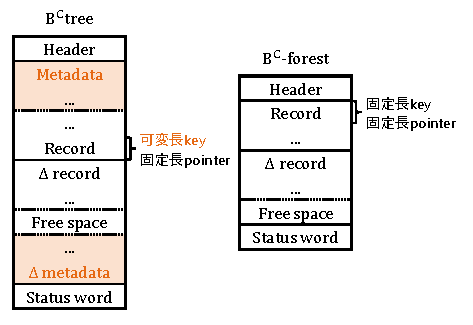
\includegraphics{./figures/inner_node.pdf}
    \caption{\Bcforest{}中間ノードにおけるレコードメタデータの除外}
    \label{fig:inner}
\end{figure}

\Bcforest{}では中間ノードはキーを8~byteで分割しているため,固定長キーとして扱うことが出来る.
また,ペイロードは子ノードへのポインタであるため固定長である.
この特性を利用し,\Bcforest{}内の\Bctree{}における中間ノード内のレコードメタデータの除外を行う.
これにより,索引層における探索性能の改善及びキャッシュ効率を改善を図る.

\subsection{葉ノードにおけるposting listの導入}

\begin{figure*}[t]
    \centering
    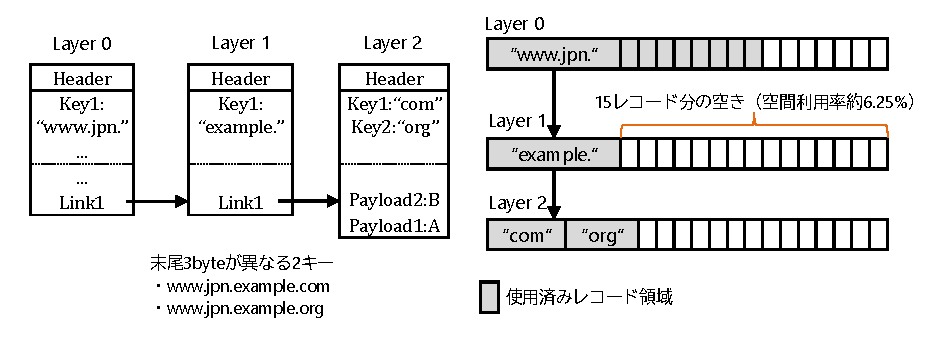
\includegraphics{./figures/memory.pdf}
    \caption{Mass木の空間利用率}
    \label{fig:memory}
\end{figure*}

Mass木においては,空間利用効率が問題となる.
\Fig{\ref{fig:memory}}は末尾3~byteが異なる19~byteの2~キーを格納したMass木の索引構造である.
先頭8~byteが共通するため,layer~1を作成する.
同様に8~16~byte目が共通するため,layer~2を作成する.
Mass木では本来,1~つのノードに最大16~個のレコードを格納することが出来る.
しかしlayer~1では,1~つのレコードしか格納されていない状態でlayer~2を作成している.
layer~1にのみ注目すると,空間利用率は約6.25~\%しかない.

\begin{figure}[t]
    \centering
    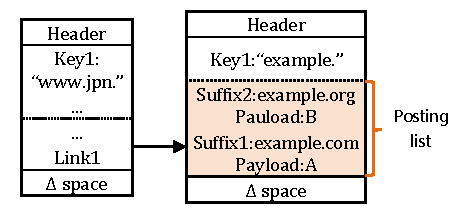
\includegraphics{./figures/posting_list.pdf}
    \caption{posting listの導入}
    \label{fig:posting_list}
\end{figure}

\Bcforest{}では空間利用率の改善として,posting listを導入する.
posting listでは,1~つのキーに対して複数のペイロードを対応付けることが出来る.
\Fig{\ref{fig:posting_list}}はposting listを導入した際の索引構造を示したものである.
layer~1においてposting list作成することで,layer~2の無駄な階層化と空間利用率の悪化を防ぐ.
なお,posting listは後述する統合時に不変領域に生成され,可変領域には生成しない.

\section{\Bcforest{}のノード操作}
\label{sec:node_operation}
本節では,\Bcforest{}のノード操作について述べる.
\Bcforest{}は読み取り操作および書き込み操作をサポートする.

ノード操作は対象ノードの特定とノード内操作の2段階に分けられる.
対象ノードの特定では,与えられた対象キーをもとに操作対象のノードを特定する.
まず,対象キーの先頭0~7~byteをもとに属するの葉ノードを根ノードから二分探索により特定する(Layer~0).
次に,葉ノード内のイミュータブル領域を二分探索し,接頭辞8~byteが共通するキーについて下層へのポインタの有無を確認する.
ポインタが無い場合,本葉ノードを挿入先の葉ノードとして特定する.
ポインタがある場合,下層の根ノードへ移動し,対象キーの8~15~byte目をもとに属する葉ノードを二分探索により特定する(Layer~1).
同様に下層ポインタの有無を確認し,本操作を下層ポインタがなくなるまで繰り返し,葉ノードを特定する.

\subsection{読み取り}
% 読み取り操作の概要とミュータブル領域での読み取り
読み取りは与えられた対象キーのペイロードを返す操作である.
操作対象の葉ノード特定後,葉ノード内の差分レコードの線形探索とイミュータブルレコードの二分探索の2ステップで読み取り操作を行う.
最新の値は差分レコード領域に書き込まれるため,まずミュータブル領域を線形探索し,一致するキーがあるか確認する.
このとき,差分レコードの数はステータスワードから読み取り,差分レコードが可視化されていなければスキップする.

% ミュータブル領域にレコードがない場合
差分レコード中に対象のレコードが存在しなければ,ノードヘッダからイミュータブルレコードの数を読み取り,二分探索によって対象キーの有無を確認する.
接頭辞8~byteが共通するキーについてposting listが存在する場合には,posting list内を線形探索し,接尾辞が一致するキーがあるか確認する.
先頭ノードが統合操作の途中である場合には,差分レコードを読み終わった時点で物理ポインタをたどり古いノードへ移動し,同様の2ステップを古いノード上で行う.

% Bc木における読み取り操作の特徴
読み取り処理はwait-freeに動作する.
上述したとおり読み取り命令は一切ノードの状態を変更せず,読み取った状態に応じて適切な手続きを選択する.
そのため,読み取り命令においてリトライなどは発生せず,有限時間内で必ず処理が終了する.

\subsection{書き込み}
% 書き込み操作の概要
書き込みは与えられた対象キーおよびペイロードを挿入する操作である.
操作対象の葉ノード特定後,posting listチェックとレコード挿入の2ステップで書き込み操作を行う.
\Bcforest{}における書き込み操作では,差分レコードのメタデータにposting listのサイズを持たせる.
これは後述する下層作成操作と書き込み操作の衝突時に,書き込み先ノードを特定するためである.

Posting listチェックでは,キーの一意性を確認する.
読み取り操作と同様にまずミュータブル領域を線形探索し,一致するキーがあるか確認する.
存在する場合,そのメタデータが持つposting listのサイズに書き込み対象のレコードのサイズを加算し,最新のサイズを計算する.
存在しない場合,イミュータブル領域を二分探索し,posting listのサイズを取得する.
以上の操作にて,取得したposting listのサイズをメタデータに入れ,\Fig{\ref{fig:bc_tree_insertion}}に示す\Bctree{}と同様の操作で挿入する.

% 書き込みができない場合の対処
以上の書き込み操作によって差分レコードを挿入していくが,挿入後の差分レコードの総数またはノード容量のしきい値を越える場合,差分レコードの構造変更操作が行われる.
しきい値の確認はステータスワードの更新時に行われ,しきい値を越えた場合はレコードの書き込み後に統合操作,構造変更操作いずれかの操作を行うか判定する.
書き込み処理はロックフリーに動作するが,後述する構造変更操作との競合によって待ち時間が発生しうる.

\section{\Bcforest{}の構造変更操作}
\label{sec:smo}
\Bcforest{}は構造変更操作として差分レコードのノードへの統合とノードの分割,下層作成操作を持つ.
構造変更操作を始める前に,新たなノードをマッピングテーブルに挿入することで,他のスレッドの待ち時間を削減する.

\subsection{統合}
% 統合操作の概要
統合操作は差分レコードの数またはノードの容量がそれぞれのしきい値を越えた場合,差分レコードとイミュータブルレコードをソートしてイミュータブル領域に反映する操作である.
本操作時に接頭辞8~byteが共通するキーを集約し,イミュータブル領域にposting list(3.2節)を作成する.
統合操作を行うことで,ミュータブル領域を確保し新たな差分レコードの挿入を受け付ける.

% 統合操作の具体的な手順
\Fig{\ref{fig:bc_tree_consolidastion}}に\Bcforest{}における統合操作を示す.
統合が必要になった場合,新たなノード領域を用意する.
そして,古いノードのステータスワードを更新後,ノードヘッダの情報から統合後に必要なイミュータブル領域を計算する.
なお,このステータスワードの更新により古いノードは全体がイミュータブルとなり,新たな差分レコードは挿入できなくなる.
次に,新たなノードにおいてステータスワードを含むヘッダ情報のみを更新した後,新規ノードとしてマッピングテーブル上の参照を更新する.
その後,古いノード上の差分レコードをイミュータブルレコードへ反映させつつ,新たなノードへレコードをコピーする.
最後に,統合後の状態でノードヘッダを更新し,新しいノードにおけるイミュータブル領域を可視化する.
この際に,後述する分割操作で用いられる分割キーを,統合後のノードのイミュータブル領域から計算する.

\begin{figure}[t]
    \centering
    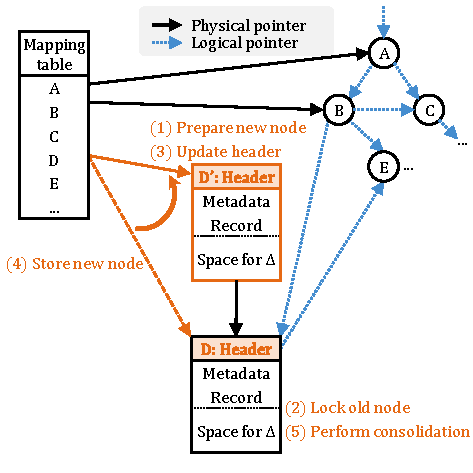
\includegraphics{./figures/Bc-consolidate.pdf}
    \caption{\Bcforest{}における統合操作}
    \label{fig:bc_tree_consolidastion}
\end{figure}

% 統合操作時の書き込みについて
統合操作を行っている際に,発生した書き込み操作は新規ノードのミュータブル領域で受け付ける.
これにより統合操作の間も,読み取り操作は新規レコードのミュータブル領域,統合前のノードのミュータブル領域およびイミュータブル領域の順でレコードを確認することで読み取り操作を実行できる.

\subsection{分割}
% 分割操作の概要
分割操作はノードの差分レコードの数またはノード容量がそれぞれしきい値を越えており,統合後も十分なミュータブル領域を確保できない場合に,そのノードのレコードを新規の2つのノードに分散させる操作である.
分割操作により,容量が一杯になったノードを2つに分け,新たな差分レコードの挿入を受け付ける.

% 分割操作の具体的な手順
\Fig{\ref{fig:bc_tree_split}}に\Bcforest{}における分割操作を示す.
構造変更操作が必要になった場合,新たなノード領域を2つ用意する.
ステータスワードの更新により対象ノード全体をイミュータブル状態にした後,レコードコピーを始める前に用意したノードをマッピングテーブルに挿入する.
これを実現するために,各ノードは自身の分割キーの位置を統合および分割操作のたびに記録する.
分割したノードの挿入後,統合操作と同様の手続きでレコードをコピーする.
分割時には,古いノードの分割キー未満の全てのレコードを左ノードにコピーする.
残りのレコード,すなわち分割キー以上の全てのレコードは右ノードにコピーする.

\begin{figure*}[t]
    \centering
    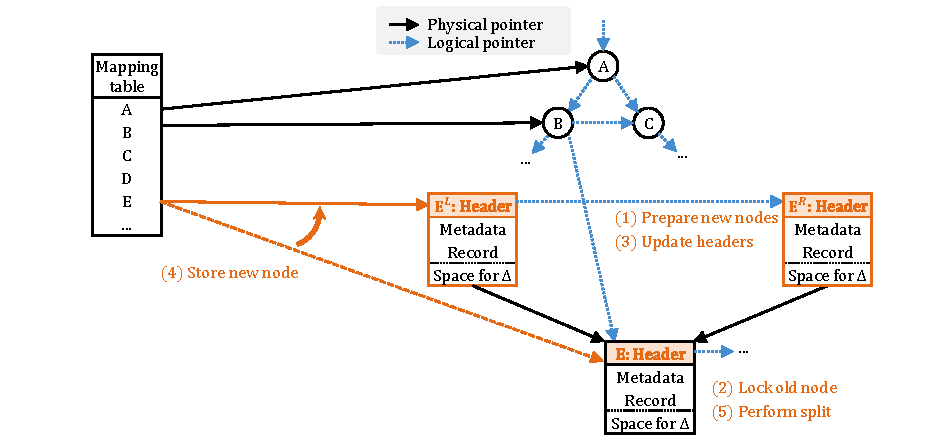
\includegraphics{./figures/Bc-split.pdf}
    \caption{\Bcforest{}における分割操作}
    \label{fig:bc_tree_split}
\end{figure*}

% 右子ノードのリンクの反映の遅延
レコードのコピー後は,親ノードに右分割ノードへのリンクを挿入することで分割操作が完了する.
このとき,親ノードへはリンクの情報のみを挿入し,反映は親ノードの統合操作時に行う.
例えば新規ノードEを挿入した際,差分レコード領域に子ノードへのリンク情報のみを追記し統合操作が行われるまでそのリンクの反映を遅延する.
つまり,索引の探索中において中間ノードでは差分レコードを確認せず,イミュータブル領域のレコードのみを検索する.

\subsection{下層作成}
% 下層作成操作の概要
下層作成操作はノードの差分レコードの数またはノード容量がそれぞれしきい値を越えており,統合後も十分なミュータブル領域を確保できない場合に,posting list内のレコードを下層に移行する操作である.
下層作成操作により,ノード内のレコードの一部を下層に移行させるとともに,新たな差分レコードの挿入を受け付ける.

\begin{figure}[t]
    \centering
    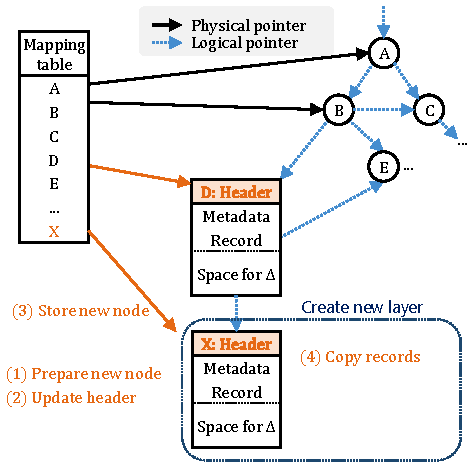
\includegraphics{./figures/layer.pdf}
    \caption{\Bcforest{}における下層作成操作}
    \label{fig:bc_tree_layer}
\end{figure}

% 下層作成操作の具体的な手順
\Fig{\ref{fig:bc_tree_layer}}に\Bcforest{}における下層作成操作を示す.
下層作成操作が必要になった場合,新たなノード領域を用意する.
レコードコピーを始める前に用意したノードをマッピングテーブルに挿入する.
下層作成操作を引き起こすきっかけとなった,posting listのレコードを新たなノードにコピーする.
この時,接尾辞の先頭8~byteをもとに必要であればposting listの作成を行う.
元ノードのposting listがあったペイロード領域に新ノードへのポインタを格納する.

% 下層作成操作時の書き込みについて
下層作成操作を行っている際に書き込み操作が発生した場合,下層生成の有無を確認する.
書き込み操作の一意性チェック時に,posting listのサイズから下層が生成されるか確認する.
生成されない場合は,元ノードに差分レコードを挿入する.
生成される場合は,下層作成操作が終わるまで書き込みはブロックされる.

\section{おわりに}
\label{sec:conclusion}
本稿では\Bctree{}にMass木と同様のトライ木構造を適応させた\Bcforest{}について提案し,その構造および操作を紹介した.
今後は提案した索引構造を実装するとともに,Mass木や近年提案されているBw木やBz木といったロックフリー索引との性能を比較検証する.